\section{Assignment 1}

The training set (\texttt{TrainingData.xlsx}) has 120 samples with four features $A$--$D$ in columns A--D and a class label
$\omega \in \{1,2,3\}$ in column E. The test set (\texttt{TestData.xlsx}) has 30 unlabelled samples. Rows are numbered by
spreadsheet row; neither file has a header row.

\subsection{Missing values and outliers}

The training set does contain missing values, three of them, each a ``?'' typed where a number should be:

\begin{table}[htbp]
\centering
\footnotesize
\caption{Incomplete training rows.}
\begin{tabular}{@{}cccc@{}}
\toprule
Row & Missing feature & Class & Remaining values ($A$, $B$, $C$, $D$) \\
\midrule
39 & A & 2 & (--, 3.3, 5.7, 2.5) \\
61 & A & 1 & (--, 3.6, 1.0, 0.2) \\
83 & D & 3 & (5.9, 3.0, 4.2, --) \\
\bottomrule
\end{tabular}
\end{table}

Outliers are there as well, three of them. Each class has to be inspected on its own, because the three classes occupy very
different ranges: feature $C$ is about 1.5 in class 1 and about 5.5 in class 2. I screened with Tukey's far-out fence, class by
class and feature by feature, so a value is flagged when it falls outside
\[
\bigl[\,Q_1 - 3\cdot \mathrm{IQR},\; Q_3 + 3\cdot \mathrm{IQR}\,\bigr],
\qquad \mathrm{IQR} = Q_3 - Q_1,
\]
where $Q_1$ and $Q_3$ are that class's lower and upper quartiles of that feature. Quartiles are interpolated linearly between
order statistics, the convention of \texttt{numpy.percentile} and \texttt{statistics.quantiles(method='inclusive')}. The data are
recorded to one or two decimal places, so the fences are computed in exact decimal arithmetic: a value sitting exactly on a
fence should not be flagged because of floating-point noise. The $3\cdot$IQR rule is a conservative screening criterion and not
a definition of what an outlier is, and the $1.5\cdot$IQR variant is discussed below.

The screening runs in a fixed order. The three incomplete rows are set aside first, not imputed and not used in the fence
calculation. For each class and each of the four features, $Q_1$, $Q_3$ and the far-out fence are then computed on the
remaining rows, every cell outside its fence is flagged, and the union of all rows holding a flagged cell is removed.

Three cells are flagged, in three different rows, so three cells and three samples are removed. The two counts coincide only
because no row contains more than one flagged cell:

\begin{table}[htbp]
\centering
\footnotesize
\caption{Far-out outliers. $\mu$ and $\sigma$ are the class's mean and standard deviation of that feature after the three rows are
removed; $z = (\text{value} - \mu)/\sigma$.}
\begin{tabular}{@{}ccccccc@{}}
\toprule
Row & Sample ($A$, $B$, $C$, $D$) & Class & Flagged value & $\mu$ ($\sigma$) & $z$ & $3\cdot$IQR fence \\
\midrule
91 & (6.3, 3.3, 16, 2.5) & 2 & $C = 16$ & 5.551 (0.586) & 17.8 & [2.70, 8.30] \\
96 & (10.6, 3.2, 1.4, 0.2) & 1 & $A = 10.6$ & 5.005 (0.328) & 17.1 & [3.80, 6.25] \\
117 & (5.7, 2.9, 4.2, 5.3) & 3 & $D = 5.3$ & 1.344 (0.196) & 20.2 & [0.30, 2.40] \\
\bottomrule
\end{tabular}
\end{table}

The other three features of each of these rows sit inside their own fences, so each row is a single-cell anomaly and not a
wholly unusual sample. The flagged values are 17 to 20 standard deviations from their class mean, well beyond anything else the
class produces. A $z$-score rule with the same class statistics ($|z| > 3$) flags exactly the same three cells, so the
conclusion does not depend on the rule chosen. Why the entry is wrong cannot be known from the data: a reading $17\sigma$ out is
consistent with a recording error, but the intended value is unrecoverable, so these rows are dropped rather than corrected.

The milder $1.5\cdot$IQR rule flags eight more borderline cells (rows 1, 26, 69, 79, 97, 98, 105, 116), with $|z|$ between 2.12
and 2.98. They sit just outside the usual range for their class, and nothing in the data suggests an error, so I kept them. That
is a judgement and not a finding: a different threshold would keep or drop a different set, which is why the threshold and the
quartile convention are stated at all.

Three methods can address the missing entries. Listwise deletion drops the incomplete samples; it invents nothing, but it is
unbiased only when the values are missing completely at random, which three cells cannot establish. With 3 of 120 samples
affected it is defensible here. Class-conditional imputation fills the entry with the mean or median of that feature over samples
of the same class; it keeps the sample but shrinks the feature's variance slightly, and it needs a known label, so an
unconditional mean would have to be used on the unlabelled test data. Model-based imputation predicts the entry from the other
features, by $k$-NN averaging or by regression on the observed ones, with EM as the likelihood-based alternative; it exploits the
correlation between features ($A$ and $C$, 0.875) but need not recover the true entry.

Three methods can address the outliers. Detection and removal flags values by a rule, a $z$-score beyond $\pm 3$ or the IQR
fences above, and deletes those samples; it works when the outliers are few and evidently wrong, and it is what I applied here.
Capping, or winsorising, replaces a value outside the fence with the nearest fence value or with a chosen percentile such as the
1st or 99th, keeping the sample but limiting its influence. The outlier can also be treated as missing and imputed (class median
or $k$-NN), or kept while the parameters are estimated with robust statistics (median and MAD), so one extreme value cannot
dominate the fit.

\subsection{Na\"ive Bayes classifier design}

As instructed, the 3 samples with missing values and the 3 outlier samples are removed, which leaves 114 training samples
(class 1: 38, class 2: 37, class 3: 39).

Each sample is a point $\mathbf{x} = (x_1, x_2, x_3, x_4) = (A, B, C, D)$, and the Bayes decision rule assigns it to the class
with the largest posterior probability
\[
P(\omega_i \mid \mathbf{x}) = \frac{p(\mathbf{x}\mid\omega_i)\,P(\omega_i)}{p(\mathbf{x})},
\qquad i = 1,2,3 .
\]
Because $p(\mathbf{x})$ is the same for every class, it is enough to compare $p(\mathbf{x}\mid\omega_i)P(\omega_i)$.

Na\"ive Bayes then assumes that, given the class, the four features are independent, so
\[
p(\mathbf{x}\mid\omega_i) = \prod_{j=1}^{4} p(x_j\mid\omega_i).
\]
This replaces one 4-dimensional density with four 1-dimensional ones, far easier to estimate from 114 samples. It is an
approximation: $A$ and $C$ correlate at 0.875 overall, and at 0.33, 0.89 and 0.74 within the three classes, so the joint density
is not a product of marginals. The classifier can still be accurate, because a decision only needs the ranking of the three
scores.

The features are continuous, so each one needs a density within each class. I took the Gaussian form because a mean and a
variance per class-feature pair specify it completely. Continuity alone does not make a variable Gaussian, and no normality check
is made here:
\[
p(x_j\mid\omega_i) = \frac{1}{\sqrt{2\pi\sigma_{ij}^2}}\,
\exp\!\left(-\frac{(x_j-\mu_{ij})^2}{2\sigma_{ij}^2}\right).
\]
With $N_i$ the number of class-$i$ samples and $N = 114$, the parameters are estimated as
\[
P(\omega_i) = \frac{N_i}{N}, \qquad
\mu_{ij} = \frac{1}{N_i}\sum_{k\in\omega_i} x_{kj}, \qquad
\sigma_{ij}^2 = \frac{1}{N_i-1}\sum_{k\in\omega_i}(x_{kj}-\mu_{ij})^2 .
\]
The unbiased variance ($N_i - 1$) is used.

\begin{table}[htbp]
\centering
\footnotesize
\caption{Fitted parameters of the three class-conditional Gaussians (114 samples after cleaning).}
\begin{tabular}{@{}cccccccccc@{}}
\toprule
\multirow{2}{*}{Class} & \multirow{2}{*}{Prior $P(\omega_i)$} & \multicolumn{2}{c}{$A$} & \multicolumn{2}{c}{$B$} & \multicolumn{2}{c}{$C$} & \multicolumn{2}{c}{$D$} \\
\cmidrule(lr){3-4}\cmidrule(lr){5-6}\cmidrule(lr){7-8}\cmidrule(lr){9-10}
 & & $\mu$ & $\sigma^2$ & $\mu$ & $\sigma^2$ & $\mu$ & $\sigma^2$ & $\mu$ & $\sigma^2$ \\
\midrule
1 & 38/114 = 0.3333 & 5.0053 & 0.1075 & 3.4079 & 0.1472 & 1.4789 & 0.0293 & 0.2553 & 0.0133 \\
2 & 37/114 = 0.3246 & 6.5541 & 0.4414 & 2.9459 & 0.0842 & 5.5514 & 0.3437 & 2.0108 & 0.0715 \\
3 & 39/114 = 0.3421 & 5.9615 & 0.2535 & 2.7821 & 0.0968 & 4.3077 & 0.2328 & 1.3436 & 0.0383 \\
\bottomrule
\end{tabular}
\end{table}

Taking the natural logarithm of $p(\mathbf{x}\mid\omega_i)P(\omega_i)$ turns the product into a sum and does not change which
class is largest:
\[
g_i(\mathbf{x}) = \ln P(\omega_i) - \sum_{j=1}^{4}\left[\tfrac{1}{2}\ln(2\pi\sigma_{ij}^2)
+ \frac{(x_j-\mu_{ij})^2}{2\sigma_{ij}^2}\right], \qquad i = 1,2,3 .
\]
The term $\tfrac{1}{2}\cdot 4\cdot\ln 2\pi = 3.6758$ is the same for all three classes, so it shifts the scores but never the
ranking. The worked example below gives the score both with and without it.

The rule is to assign $\mathbf{x}$ to $\omega_k$ where $k = \arg\max_i g_i(\mathbf{x})$, with a tie broken towards the smaller
class index (no test sample ties). Each $g_i$ is quadratic in $\mathbf{x}$ with a diagonal covariance matrix, so the decision
boundaries are quadratic surfaces in four dimensions. On the 114 cleaned training samples the classifier is 95.6\% correct,
which is a resubstitution figure and therefore optimistic, since every sample helped fit the parameters that then classify it:

\begin{table}[htbp]
\centering
\footnotesize
\caption{Na\"ive Bayes confusion matrix on the 114 cleaned training samples (rows = true class, columns = predicted class).}
\begin{tabular}{@{}ccccc@{}}
\toprule
True & $\rightarrow 1$ & $\rightarrow 2$ & $\rightarrow 3$ & Recall \\
\midrule
1 & 38 & 0 & 0 & 38/38 = 100\% \\
2 & 0 & 34 & 3 & 34/37 = 91.9\% \\
3 & 0 & 2 & 37 & 37/39 = 94.9\% \\
\bottomrule
\end{tabular}
\end{table}

All five errors are confusions between classes 2 and 3: rows 12, 23 and 85 (class 2 read as class 3) and rows 56 and 89 (class 3
read as class 2). Class 1 is never confused with anything, which is what its well-separated $C$ and $D$ values predict
(Figure~\ref{fig:cd}).

Because 95.6\% is measured on the samples used for fitting, a held-out estimate is also reported. Refitting the classifier 114
times, each time on 113 samples and testing on the omitted one (leave-one-out), gives 94.7\%:

\begin{table}[htbp]
\centering
\footnotesize
\caption{Leave-one-out confusion matrix for the same classifier (each row refits without that sample).}
\begin{tabular}{@{}cccc@{}}
\toprule
True & $\rightarrow 1$ & $\rightarrow 2$ & $\rightarrow 3$ \\
\midrule
1 & 38 & 0 & 0 \\
2 & 0 & 34 & 3 \\
3 & 0 & 3 & 36 \\
\bottomrule
\end{tabular}
\end{table}

Only one prediction changes (row 56 becomes an error, giving 108/114 = 94.7\%), because its neighbours then supply slightly
different variances. The model has only $2 + 12 + 12 = 26$ free parameters for 114 samples, which is why the two figures are so
close.

As a worked example, take test sample 11, $\mathbf{x} = (6.0, 2.2, 5.0, 1.5)$. Its per-feature penalty terms
$\tfrac{1}{2}\ln(2\pi\sigma^2) + (x-\mu)^2/(2\sigma^2)$ come out as follows:

\begin{table}[H]
\centering
\footnotesize
\caption{Class scores for test sample 11. $\tilde{g}$ is the reduced discriminant (without the 3.6758 constant); $P$ is the
posterior of the class.}
\begin{tabular}{@{}ccccccccc@{}}
\toprule
Class & $\ln P(\omega_i)$ & $A$ & $B$ & $C$ & $D$ & $g_i(\mathbf{x})$ & $\tilde{g}_i(\mathbf{x})$ & $P(\omega_i\mid\mathbf{x})$ \\
\midrule
1 & $-1.0986$ & 4.4046 & 4.9158 & 210.9042 & 56.7900 & $-278.11$ & $-274.44$ & 0.00\% \\
2 & $-1.1253$ & 0.8578 & 2.9853 & 0.8272 & 1.4237 & $-7.22$ & $-3.54$ & 2.71\% \\
3 & $-1.0726$ & 0.2356 & 1.5016 & 1.2195 & $-0.3928$ & $\mathbf{-3.64}$ & $\mathbf{0.04}$ & $\mathbf{97.29\%}$ \\
\bottomrule
\end{tabular}
\end{table}

For example, for class 3 and feature $A$: $\tfrac{1}{2}\ln(2\pi\times 0.2535) + (6.0-5.9615)^2/(2\times 0.2535) = 0.2327 +
0.0029 = 0.2356$. The four terms sum to 2.564, so $g_3 = -1.0726 - 2.564 = -3.64$, the largest of the three scores: sample 11
lands in class 3. Class 1 loses by a wide margin, mostly because $C = 5.0$ is far from class 1's mean of 1.48 and its variance
is small (0.0293), so the squared distance is divided by a small number.

\subsection{Predicted class labels of the test data}

\begin{table}[htbp]
\centering
\footnotesize
\caption{Discriminant values and predictions for the 30 test samples. $P$ is the posterior probability of the predicted class;
margin is the gap between the best and the second-best score.}
\begin{tabular}{@{}rrrrrrrrrrr@{}}
\toprule
Test \# & $A$ & $B$ & $C$ & $D$ & $g_1$ & $g_2$ & $g_3$ & Predicted & $P$ (\%) & margin \\
\midrule
1 & 4.8 & 3.1 & 1.6 & 0.2 & 0.34 & $-50.56$ & $-36.53$ & \textbf{1} & 100.0 & 36.87 \\
2 & 5.1 & 3.5 & 1.4 & 0.3 & 0.97 & $-51.05$ & $-37.03$ & \textbf{1} & 100.0 & 38.00 \\
3 & 4.8 & 3.0 & 1.4 & 0.1 & $-0.55$ & $-55.39$ & $-41.78$ & \textbf{1} & 100.0 & 41.23 \\
4 & 5.7 & 3.8 & 1.7 & 0.3 & $-2.45$ & $-48.49$ & $-34.84$ & \textbf{1} & 100.0 & 32.39 \\
5 & 5.5 & 4.2 & 1.4 & 0.2 & $-2.27$ & $-59.89$ & $-46.57$ & \textbf{1} & 100.0 & 44.30 \\
6 & 5.0 & 3.4 & 1.5 & 0.2 & 1.10 & $-52.06$ & $-38.33$ & \textbf{1} & 100.0 & 39.43 \\
7 & 4.6 & 3.1 & 1.5 & 0.2 & 0.01 & $-52.56$ & $-38.71$ & \textbf{1} & 100.0 & 38.72 \\
8 & 5.8 & 4.0 & 1.2 & 0.2 & $-4.35$ & $-59.00$ & $-46.06$ & \textbf{1} & 100.0 & 41.71 \\
9 & 5.0 & 3.6 & 1.4 & 0.2 & 0.88 & $-54.57$ & $-41.04$ & \textbf{1} & 100.0 & 41.91 \\
10 & 4.6 & 3.4 & 1.4 & 0.3 & 0.28 & $-52.38$ & $-38.53$ & \textbf{1} & 100.0 & 38.81 \\
11 & 6.0 & 2.2 & 5.0 & 1.5 & $-278.11$ & $-7.22$ & $-3.64$ & \textbf{3} & 97.3 & 3.58 \\
12 & 6.5 & 3.2 & 5.1 & 2.0 & $-347.27$ & $-1.99$ & $-8.98$ & \textbf{2} & 99.9 & 6.99 \\
13 & 7.7 & 3.0 & 6.1 & 2.3 & $-554.42$ & $-3.83$ & $-25.58$ & \textbf{2} & 100.0 & 21.75 \\
14 & 6.9 & 3.2 & 5.7 & 2.3 & $-476.52$ & $-2.44$ & $-19.27$ & \textbf{2} & 100.0 & 16.84 \\
15 & 7.9 & 3.8 & 6.4 & 2.0 & $-565.89$ & $-8.73$ & $-28.32$ & \textbf{2} & 100.0 & 19.59 \\
16 & 6.5 & 3.0 & 5.2 & 2.0 & $-360.23$ & $-1.50$ & $-8.69$ & \textbf{2} & 99.9 & 7.18 \\
17 & 6.2 & 2.8 & 4.8 & 1.8 & $-284.42$ & $-2.70$ & $-3.89$ & \textbf{2} & 76.6 & 1.19 \\
18 & 6.7 & 2.5 & 5.8 & 1.8 & $-423.21$ & $-2.91$ & $-9.52$ & \textbf{2} & 99.9 & 6.61 \\
19 & 6.2 & 3.4 & 5.4 & 2.3 & $-424.60$ & $-3.29$ & $-17.12$ & \textbf{2} & 100.0 & 13.83 \\
20 & 6.5 & 3.0 & 5.5 & 1.8 & $-375.26$ & $-1.64$ & $-7.12$ & \textbf{2} & 99.6 & 5.49 \\
21 & 6.8 & 3.0 & 5.5 & 2.1 & $-417.93$ & $-1.45$ & $-12.69$ & \textbf{2} & 100.0 & 11.24 \\
22 & 5.8 & 2.7 & 4.1 & 1.0 & $-141.53$ & $-12.51$ & $-2.25$ & \textbf{3} & 100.0 & 10.26 \\
23 & 6.8 & 2.8 & 4.8 & 1.4 & $-252.47$ & $-4.93$ & $-2.49$ & \textbf{3} & 92.0 & 2.44 \\
24 & 6.7 & 3.1 & 4.4 & 1.4 & $-207.27$ & $-6.00$ & $-2.19$ & \textbf{3} & 97.8 & 3.81 \\
25 & 5.2 & 2.7 & 3.9 & 1.4 & $-149.85$ & $-10.31$ & $-2.11$ & \textbf{3} & 100.0 & 8.20 \\
26 & 5.7 & 2.6 & 3.5 & 1.0 & $-93.78$ & $-16.10$ & $-3.78$ & \textbf{3} & 100.0 & 12.32 \\
27 & 5.6 & 2.5 & 3.9 & 1.1 & $-130.06$ & $-13.28$ & $-2.33$ & \textbf{3} & 100.0 & 10.94 \\
28 & 5.5 & 2.5 & 4.0 & 1.3 & $-152.15$ & $-10.77$ & $-1.59$ & \textbf{3} & 100.0 & 9.18 \\
29 & 5.0 & 2.0 & 3.5 & 1.0 & $-96.05$ & $-22.61$ & $-8.46$ & \textbf{3} & 100.0 & 14.15 \\
30 & 6.4 & 3.2 & 4.5 & 1.5 & $-221.88$ & $-5.14$ & $-2.22$ & \textbf{3} & 94.9 & 2.93 \\
\bottomrule
\end{tabular}
\end{table}

So the 30 test samples fall into three groups: samples 1 to 10 go to class 1, samples 12 to 21 to class 2, and sample 11 with
samples 22 to 30 to class 3.

Class 1 is separated from the other two by a wide margin, mostly through features $C$ and $D$. The closest decisions are
sample 17 ($g_2 - g_3 = 1.19$, so $P(\omega_2\mid\mathbf{x}) = 76.6\%$), sample 23 (margin 2.44, $P = 92.0\%$) and sample 30
(margin 2.93, $P = 94.9\%$); the worked example, sample 11, is only the fourth closest (margin 3.58). All three of the closest
samples lie where classes 2 and 3 overlap in $C$, which is visible in Figure~\ref{fig:cd}. These are model scores; with no test
labels, nothing here measures accuracy.

\begin{figure}[H]
\centering
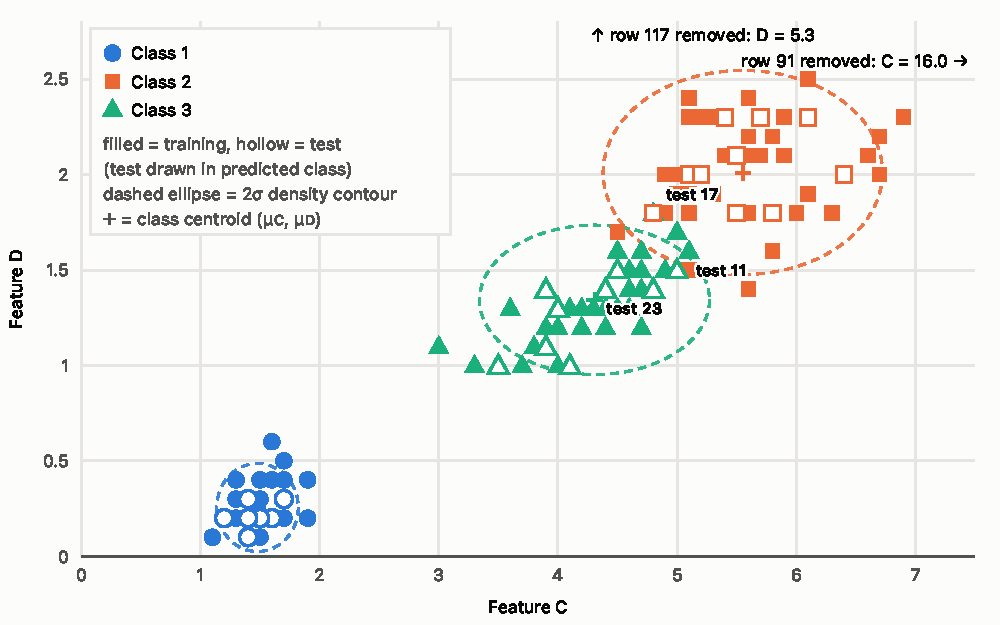
\includegraphics[width=\linewidth]{figures/fig1.pdf}
\caption{Features $C$ and $D$ for the 114 cleaned training samples (filled) and the 30 test samples (hollow, drawn in their
predicted class), with the $2\sigma$ density contour of each fitted class Gaussian and its centroid marked by a cross. Class 1
is well separated; classes 2 and 3 overlap, and that overlap is where the closest test decisions (17, 23, 30) and the five
training errors lie. Row 91's outlier ($C = 16.0$) and row 117's ($D = 5.3$) fall outside the plotted range, and row 96's
outlier is in feature $A$.}
\label{fig:cd}
\end{figure}
